\subsection{MDP-Tetris \label{sec:MDPTetris}}

As described earlier, MDPTetris is used as the 
platform for emulating Tetris controllers. The source code for the 
platform is freely available at \url{http://mdptetris.gforge.inria.fr/doc/index.html}.
The software implements the simplified version of Tetris as described in 
section \ref{sec:learningTetris} and is written in C. The code depends on
the GNU Scientific Library\footnote{\url{http://www.gnu.org/software/gsl/}} and
the OpenGL Utility 
Library GLUT/freeGLUT\footnote{\url{http://freeglut.sourceforge.net/}}.
The library implements a set of executable programs. These programs 
allows execution of agents with fixed policies and visualizations
of the Tetris games using OpenGL.\\
\\
The core application of the source code is a function that allows evaluation of 
a controller. This function accepts the configuration of the game one wishes to play,
simulates game, and returns the number of lines cleared by the agent during the game.
The configuration of the game is mostly done through reading data files that describes 
different qualities of the game. The feature set is read from a file,
like the one seen in figure \ref{fig:featfile}. This file defines which features that are to be 
considered by the controller by indices. Each of these indices map to a feature function 
implemented in the MDPTetris code. The pieces that occur in the game are also read from a file,
which in our case, is just a file that contains the 7 regular pieces from the ordinary game
(see figure \ref{fig:TetrisPieces}). Later in the experiments however, a harder version of Tetris
is discussed, which is harder due to more frequent occurrence of difficult to place pieces.
To increase the likelihood of these pieces, the piece configuration file was altered to
contain more of the difficult pieces, thus making them occur more often.\\
\\
To perform the actual optimization of the Tetris agents, the Shark library has been applied
with it's implementation of CMA algorithm and with our own implementation of the Cross Entropy (now a part of Shark,
see appendix \ref{app:crossEntropyCode}).\\
The two optimization algorithms in shark both inherits from the abstract class\\ 
\lstinline$AbstractSingleObjectiveOptimizer<RealVector>$. This superclass defines the
abstract interface for an optimizer that can be applied to problems of finding 
solutions of the type \lstinline$RealVector$ that models a real valued vector.
The objective functions are in Shark implemented by writing a class that inherits 
the \lstinline$SingleObjectiveFunction$ which is an interface for an objective function 
that accepts a single real valued vector and returns a real value indicating how well the supplied
vector evaluates against the underlying function. In our code, we implemented the class names 
\lstinline$MDPTetris$ that inherits the abstract \lstinline$SingleObjectiveFunction$ class.
Thus, our implementation of the objective function offers an abstraction that, to Shark, masks
the actual implementation and configuration of Tetris. The effect of this abstraction is that 
no code from Shark need to be aware of any details of the actual function, in this case
Tetris, that is being optimized.\\
\\
The \lstinline$MDPTetris$ objective function is adjustable in terms of Tetris board size, piece 
configuration file and feature set. When loading the feature set, the dimensionality of 
the function is set to match the number of features which allows the optimizer to 
scale its search space accordingly.
\begin{figure}[h!]
\begin{center}
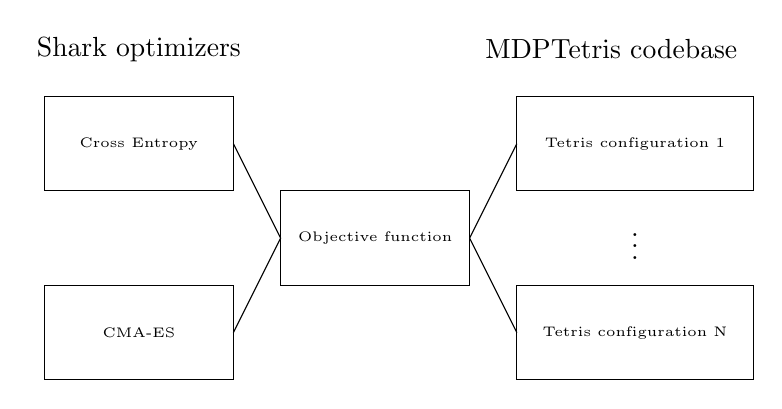
\begin{tikzpicture}[scale=0.6]
\draw  (0,0) rectangle (4,2);
\node at (2,1) {\tiny Objective function};
\draw  (-5,4) rectangle (-1,2);
\node at (-3,3) {\tiny Cross Entropy};
\draw  (-5,0) rectangle (-1,-2);
\node at (-3,-1) {\tiny CMA-ES};
\draw  (5,4) rectangle (10,2);
\draw  (5,0) rectangle (10,-2);
\node at (7.5,1) {$\vdots$};
\node at (7.5,3) {\tiny Tetris configuration 1};
\node at (7.5,-1) {\tiny Tetris configuration N};
\draw (-1,3) -- (0,1) -- (-1,-1);
\draw (5,3) -- (4,1) -- (5,-1);
\node at (-3,5) {Shark optimizers};
\node at (7,5) {MDPTetris codebase};
\end{tikzpicture}
\end{center}
\caption{Fusion of Shark and MDPTetris}
\end{figure}


The source code of the MDPTetris source code 
is accompanied with files that describe the
various existing features, that is files that defines 
the commonly used feature sets. As described, these files contains the identifiers of 
each feature to use, as well as two numbers respectively describing 
the agents reward function and how to evaluate a 'game over' state. 
The number for the reward function has remained unchanged at $0$ 
during all experiments. The "game-over" evaluation was for the
Bertsekas feature set initially set to $0$. Setting the 
"game-over" evaluation to $0$ means that the agent will not 
distinguish between regular moves and moves that results in losing
the game. If this setting remains at 0, the agent will always consult the
feature functions to rank it's moves, yet setting this value to $-1$
the agent will always, regardless of feature functions, rank moves that ends
the game the lowest.
When running the experiments with this setting as $0$, a large portion
of the agents never exceeded a zero mean score. This occurs presumingly 
due to all agents failing quickly giving the optimization algorithm no 
useful feedback. However, setting the value
to $-1$, meaning that a "game-over" move yields $-\infty$ reward, 
none of the experiments got stuck on only zero scores. An example
of the layout of the feature file can be seen in figure \ref{fig:featfile}.
\begin{figure}[h!]
\centering
\begin{lstlisting}
0    <- Describes the reward function
-1   <- Actions leading to game over is avoided at all cost
22   <- The policy contains 22 features
8 0  <- The feature with id 8 initially has weight 0
...  <- The remaining 21 features
\end{lstlisting}
\caption{Example of a file that describes a feature set. \label{fig:featfile}}
\end{figure}

\subsubsection{Game complexity \label{HardTetris}}
\comment{Allerede nævnt i forrige afsnit - kort dog}\\
In order to reduce the runtime of experiments, to allow us more experiments in the evaluations, we can increase the "difficulty" of Tetris, by adjusting either the board size and/or adjusting the frequency of certain pieces. This has also been described before by Amine Boumaza, \citep{boumaza2009}.\\
To increase the difficulty of the game,
in our so-called "Hard" Tetris, the s-block and z-block appear twice as often 
as the other pieces.

\begin{figure}[H]
\begin{center}
\includegraphics[scale=0.6]{img/Pieces}
\end{center}
\caption{Regular Tetris pieces \label{fig:TetrisPieces}}
\end{figure}

We want to test if altering the game complexity has an impact on the performance of the algorithms,
therefore we will to test the two algorithms with Bertsekas/Tsitsiklis featureset, using Normal Tetris and Hard Tetris.\\

\textbf{Results}\\
In the following figure is depicted the mean results of 30 individual experiments using Cross Entropy and CMA, applied to both Hard Tetris and Normal Tetris. The general settings of the experiments can be seen in the appendix section, \ref{AppendixGameComplexity}.

\begin{table}[H]
\centering
\small
\begin{tabular}{l l r r r r r}
Tetris Type & Optimizer & mean & Q1 & Q2 & Q3\\
\hline
Hard & Cross Entropy & $1633.607$ & $1357.170$ & $1606.565$ & $1938.71$\\
Normal & Cross Entropy & $100059.463$ & $79357.440$ & $105999.500$ & $111047.500$\\
Hard & CMA & $449.352$ & $201.850$ & $300.300$ & $529.350$\\
Normal & CMA & $49760.161$ & $42528.740$ & $49915.700$ & $67764.729$\\
\end{tabular}
\caption{Experiment testing game Normal Tetris against Hard Tetris}
\end{table}

\begin{figure}[H]
\centering
\includegraphics[scale=1]{data/complexity/mean/PlotFile.pdf}
\caption{Experiment testing Normal Tetris against Hard Tetris}
\end{figure}

\textbf{Analysis and discussion}\\
The results indicate that using Hard Tetris does not impact the general development of the algorithms. Though the score values are different, the development of the algorithms remain the same. CMA converges faster than Cross Entropy, however, Cross Entropy achieves a higher score convergence.\\
Meaning we are able to use the harder Tetris for further experiments. From the graph it appears that the harder Tetris simply shifts the score compared to normal Tetris.\\
\comment{skal der komme en reference til \citep{boumaza2009}, som dog ikke har lavet nogen eksperimenter, men siger at det er ok at bruge}


\subsubsection{Comparison of featuresets  \label{compoffeatureset}}
\comment{find reference til beskrivelse af dellachie og bertsekas feature set}\\
As described in section \ref{ConfigureTetrisBackground}, there are different kind of
feature sets which impacts the performance of the agents.\\
For our comparison experiments between CMA and Cross Entropy,
we are going to use the Bertsekas/Tsitsiklis feature set, since other researchers report
a lower score with the Bertsekas/Tsitsiklis feature set compared with the Dellacherie featureset \citep{thiery:09}.\\
Unlike the \citep{thiery:09} experiments, we don't want to maximize the
final score, but rather maximize the score with the lowest possible number of 
games evaluated.\\
It's important to note that we are not going to conduct comparison experiments with different
feature sets in the same experiment, since the algorithms needs to be on equal terms for an unbiased comparison.\\
\\
We want to test whether the feature set has an impact on the performance of the algorithms,
therefore we want to test the two algorithms with both the Dellacherie and Bertsekas/Tsitsiklis featureset.\\
From the game complexity section \ref{HardTetris}, we have verified that using Hard Tetris
\citep{boumaza2009} does not have an impact on the development of the two algorithms.
Therefore, to prevent long runtimes, the games are simulated
using Hard Tetris.\\

\textbf{Results}\\
In the following figures the mean results of 30 runs of both CMA and Cross 
Entropy is presented. The settings for Cross Entropy remains at constant noise
with a noise term of $z_t = 4$ and an initial sigma $\sigma_0 = 100$, 
and the CMA with $\sigma_0 = 1$.\\
\\
Figure \ref{fig:featuresetCompareBertsekas} shows the experiment with the 
Bertsekas feature set. The algorithms behave mostly the same as seen before.
Namely that CMA converges faster than Cross Entropy, 
but is eventually outperformed.

\begin{figure}[H]
\includegraphics[scale=1]{plots/plotBertsekasCmaVsCEHardTetris}
\caption{Comparison between CMA-ES and Cross Entropy 
using hard Tetris and the Bertsekas featureset 
\label{fig:featuresetCompareBertsekas}}
\end{figure}

When using the Dellacherie feature set a similar behaviour is observed.
However, the convergence seems to occur earlier and with a higher score
(figure \ref{fig:featuresetCompareDellacherie}).

\begin{figure}[H]
\includegraphics[scale=1]{plots/plotDellCmaVsCEHardTetris}
\caption{Comparison between CMA-ES and Cross Entropy 
using hard Tetris and the Dellacherie featureset
\label{fig:featuresetCompareDellacherie}}
\end{figure}

\textbf{Analysis and discussion}\\
\comment{more discussion?}\\
The experiment with different feature sets indicates that the behaviour of the algorithms
is not heavily dependant on the feature set.
It appears that changing the feature set simple shifts the score, but does not affect the development of the graphs.\\
Therefore, we conclude that changing the feature set does not invalidate
the comparison of the two optimization algorithms.

